% draft会跳过文档中的所有图片。正式导出时需要删掉draft参数。
\documentclass[12pt, a4paper, oneside]{ctexart}

\usepackage{amsmath}
\usepackage{amssymb}
\usepackage{amsopn}
\usepackage{bm}
\usepackage{graphicx}
\usepackage{mathrsfs}
\usepackage{geometry}
\usepackage{framed}
\usepackage{color}
\usepackage{caption}
\usepackage{listings}
\usepackage{fancyhdr}
\usepackage{booktabs}
\usepackage{makecell}
\usepackage{indentfirst}
\usepackage{authblk}
\usepackage{multicol}
% \usepackage{draftwatermark}       % 需要应用水印时取消注释
\usepackage{enumitem}
\usepackage[hidelinks]{hyperref}
\usepackage{tikz}
\usepackage{ulem}
\usetikzlibrary{positioning, shapes.geometric}

% 分栏线宽
\columnseprule=0.4pt

% 定制第二级无序列表的点样式
\setlist[itemize,2]{label=$\diamond$}

% 页边距
\geometry{a4paper, scale=0.8}

\pagestyle{fancy}

% 调整页眉高度,用于去除警告
\setlength{\headheight}{25pt}

\fancyhf{}      % 清空页眉页脚设置
\fancyhead[L] {
    % 工大计算机系logo
    
\includegraphics[height=7mm]{../../../share/images/logo1.jpg}
}
\fancyhead[C]{《数据结构》复习}
\fancyhead[R]{\leftmark}    % 右侧页眉:当前章标题

% 页脚居中放置页码
\fancyfoot[C]{\thepage}

% 设置章节标题自动编号的格式
\ctexset{
  section/number=\chinese{section},
%   subsection/name={,},
%   subsection/number=\chinese{subsection}
}

% 行距。ctexart默认值为1.3
\linespread{1.2}

\lstset{
  language=c,
  basicstyle=\ttfamily,
  frame=single,
  numbers=left
}

% \SetWatermarkText{Eslzzyl整理}            % 设置水印内容
% \SetWatermarkLightness{0.9}             % 设置水印透明度 0-1
% \SetWatermarkScale{0.8}                   % 设置水印大小 0-1

\renewcommand{\headrulewidth}{1pt}  %页眉线宽,设为0可以去页眉线
\renewcommand{\footrulewidth}{1pt}  %脚注线的宽度

\definecolor{shadecolor}{RGB}{241, 241, 255}

\title{
    
\includegraphics[width=0.3\textwidth]{../../../share/images/hfut-badge.pdf}
    
    \vspace{20pt}
    《数据结构》总复习
}
\author{Eslzzyl}
\date{\today}

\newcounter{problemname}
\newenvironment{problem}{\begin{shaded}\stepcounter{problemname}\par\noindent\textbf{例题\arabic{problemname}. }}{\end{shaded}\par}
\newenvironment{solution}{\begin{shaded}\par\noindent\textbf{解答:}}{\end{shaded}\par}
% \newenvironment{solution}{\par\noindent\textbf{答案. }}{\par}
% \newenvironment{note}{\par\noindent\textbf{例题\arabic{problemname}的注记. }}{\\\par}
\newenvironment{note}{\par\noindent\textbf{注记. }}{\par}

\begin{document}

\maketitle
\newpage
\tableofcontents
\vspace{20pt}
% 如果在目录处有备注,可以写在这里。

\newpage

\section{绪论}

\subsection{数据结构的基本概念}

\subsubsection{基本概念和术语}

\begin{itemize}
  \item {\bf 数据},是信息的载体,是计算机程序加工的原料。
  \item {\bf 数据元素},是数据的基本单位,如一个学生记录。可由若干个数据项组成,如包含学号、姓名、性别等数据项。
  \item {\bf 数据对象},是具有\textbf{相同性质}的数据元素的集合。
  \item {\bf 数据类型},是一个值的集合和定义在此集合上的一组操作的总称。
  \begin{itemize}
    \item 原子类型:不可再分的数据类型。
    \item 结构类型:可以再分的数据类型。
    \item 抽象数据类型
  \end{itemize}
  \item {\bf 数据结构},是相互之间存在一种或多种特定关系的数据元素的集合。数据结构包括三方面内容:
  \begin{itemize}
    \item 逻辑结构,决定算法的设计
    \item 存储结构,又叫映像,决定算法的实现
    \item 数据的运算
  \end{itemize}
\end{itemize}

\subsubsection{数据结构三要素}

\begin{enumerate}
  \item {\bf 数据的逻辑结构}
  
  \begin{figure}[h]
    \centering
    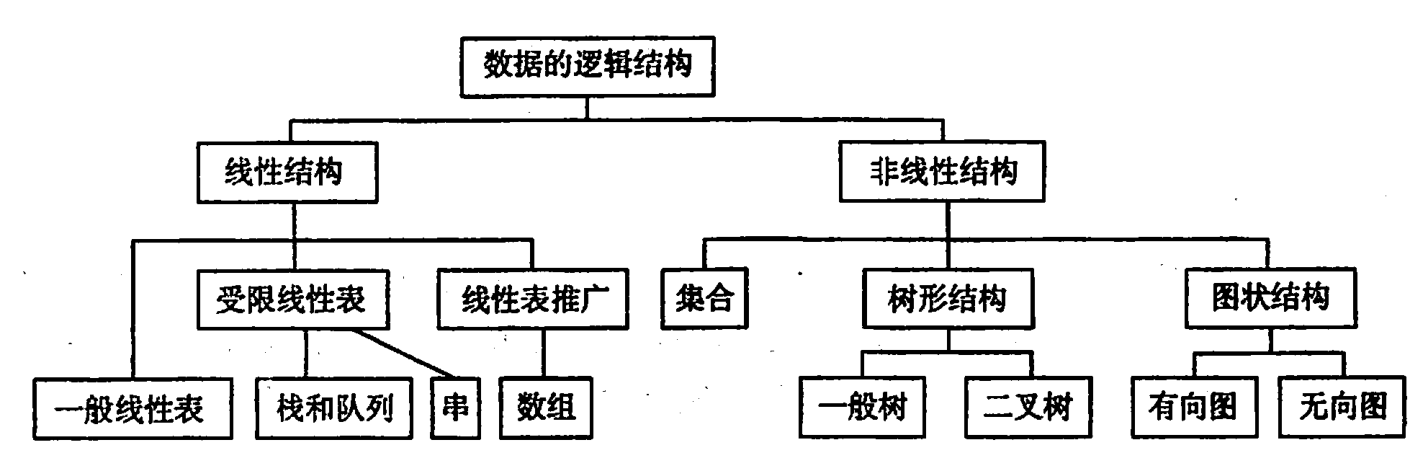
\includegraphics[width=0.7\textwidth]{./images/logical-structure.png}
    \caption{数据的逻辑结构}
    \label{logical-structure}
  \end{figure}
  
  逻辑结构可分为线性结构和非线性结构。见图\ref{logical-structure}。

  \begin{itemize}
    \item {\bf 集合}:结构中的元素之间除了“同属一个集合”之外,没有别的关系。
    \item {\bf 线性结构}:元素之间存在一对一的关系。
    \item {\bf 树形结构}:元素之间存在一对多的关系。
    \item {\bf 图状结构或网状结构}:元素之间存在多对多的关系。
  \end{itemize}

  \item {\bf 数据的存储结构}
  
  存储结构是用计算机语言实现的逻辑结构。
  \begin{itemize}
    \item {\bf 顺序存储}
    \item {\bf 链式存储}
    \item {\bf 索引存储}
    \item {\bf 散列存储}
  \end{itemize}

  \item {\bf 数据的运算}
\end{enumerate}

\subsection{算法和算法评价}

\subsubsection{算法的基本概念}

算法(Algorithm)是对特定问题求解步骤的一种描述。有以下5个重要特性:
\begin{enumerate}
  \item {\bf 有穷性},算法必须在有限个步骤之后结束,且每一步必须消耗有限的时间。
  \item {\bf 确定性},同一个算法对同一个输入必定得出相同的输出。
  \begin{itemize}
    \item 随机类算法不违反确定性,因为计算机是伪随机,对于同一个随机种子,生成的随机数序列总是一致的。
  \end{itemize}
  \item {\bf 可行性}
  \item {\bf 输入},算法有0个或更多个输入。
  \item {\bf 输出},算法有一个或更多个输出。
\end{enumerate}

设计一个好的算法应该考虑:
\begin{itemize}
  \item 正确性
  \item 可读性
  \item 健壮性
  \item 高效率与低存储量需求
\end{itemize}

\subsubsection{算法效率的度量}

\begin{enumerate}
  \item {\bf 时间复杂度}
  
  通常采用算法中基本运算的频度来分析时间复杂度。

  一般总是考虑在最坏情况下的时间复杂度。

  常见的渐进时间复杂度:
  \begin{equation*}
    O(1)<O(\log_2 n)<O(n)<O(n\log_2 n)<O(n^2)<O(n^3)<O(n!)<O(n^n)
  \end{equation*}
  \item {\bf 空间复杂度}
  
  算法\textbf{原地工作}是指算法所需的辅助空间为常量,即$O(1)$。
\end{enumerate}

\section{线性表}

\subsection{线性表的定义和基本操作}

\subsubsection{线性表的定义}

线性表是具有相同数据类型的$n$($n\geq 0$)个数据元素的有限序列,其中$n$为表长。
\begin{equation*}
  L=(a_1,a_2,\cdots,a_i,a_{i+1},\cdots,a_n)
\end{equation*}

线性表的特点:
\begin{itemize}
  \item 表中元素的个数有限。
  \item 元素具有逻辑上的顺序性。
  \item 元素都是数据元素。
  \item 元素的数据类型都相同,占有相同大小的存储空间。
  \item 元素具有抽象性,不关心元素中保存的是什么内容。
\end{itemize}

线性表是逻辑结构,顺序表和链表是物理结构。

\subsubsection{线性表的基本操作}

\begin{itemize}
  \item \verb|InitList(&L)|:初始化表,构造一个空的线性表。
  \item \verb|Length(L)|:返回表的长度
  \item \verb|LocateElem(L, e)|:按值查找
  \item \verb|GetElem(L, i)|,按位置查找
  \item \verb|ListInsert(&L, i, e)|:插入
  \item \verb|ListDelete(&L, i, &e)|:删除
  \item \verb|PrintList(L)|:输出表
  \item \verb|Empty(L)|:判空,空返回\verb|true|
  \item \verb|DestroyList(&L)|:销毁表
\end{itemize}

\subsection{线性表的顺序表示}

注意线性表的下标是从1开始算,数组的下标是从0开始算。

时间复杂度分析(平均):
\begin{itemize}
  \item 随机访问:$O(1)$
  \item 插入:$O(n)$
  \item 删除:$O(n)$
  \item 顺序查找:$O(n)$
\end{itemize}

\subsection{线性表的链式表示}

链表往往引入头结点,有如下好处:
\begin{itemize}
  \item 在链表的第一个位置上的操作和其他位置一致,无需进行特殊处理。
  \item 无论链表是否为空,头指针都指向一个节点,这样空表和非空表的处理得到了统一。
\end{itemize}

建立新链表:
\begin{itemize}
  \item 头插:在头部插入节点,形成的链表的顺序是反的。
  \item 尾插:在尾部插入节点,顺序正常,但需要添加额外的尾指针。
\end{itemize}

时间复杂度分析:
\begin{itemize}
  \item 建立新链表(头插/尾插):$O(n)$
  \item 按序号查找:$O(n)$
  \item 按值查找:$O(n)$
  \item 按值删除:主要耗费在查找上。$O(n)$
  \item 按值插入:同上
  \item 求表长:$O(n)$
\end{itemize}

插入元素时,往往要先找到元素所在的位置,然后执行后插。查找的复杂度是$O(n)$,后插的复杂度仅为$O(1)$。因此:
\begin{itemize}
  \item 当给出插入位置的值时,总复杂度为$O(n)$;
  \item 当给出插入位置的地址时,总复杂度为$O(1)$。
\end{itemize}

有时需要前插,此时要找到目标结点的前面一个节点。对于单链表,必须按照顺序向后查找。此时无论给出的是值还是地址,总复杂度都为$O(n)$;但有一种优化方法:在目标结点的后继插入,然后交换目标结点和新插入结点的值。此时已知地址时,总复杂度为$O(1)$。

类似地,删除结点时,必须得知前驱结点,这样才能正确设置链接关系。但如果直接将后继结点的值赋予待删除结点,然后删除后继结点,这样也能有$O(1)$时间复杂度。

\subsubsection{双链表}

\subsubsection{循环链表}

循环单链表的判空条件不是头结点的指针是否为空,而是它是否等于头指针。

循环单链表少用头指针而多用尾指针。因为尾指针的\verb|next|就是头结点。

\subsubsection{静态链表}

静态链表是用数组实现的链表。不太方便,但是适合没有指针的语言。

\subsubsection{顺序表的链表的比较}

\begin{itemize}
  \item {\bf 存取(读写)方式}
  
  顺序表既能顺序读取,又能随机读取;链表只能顺序读取。

  \item {\bf 逻辑结构与物理结构}
  
  逻辑上都是线性表,但顺序表的结点物理上也是连续的,链表的结点靠指针维持连续性。

  \item {\bf 查找、插入和删除操作}
  \begin{itemize}
    \item 对于按值查找,若表无序,则二者均为$O(n)$;若有序,则顺序表可用二分查找,$O(\log_2 n)$。
    \item 对于按序号查找,顺序表可以随机访问,$O(1)$;链表则为$O(n)$。
  \end{itemize}

  对于插入和删除操作,顺序表的平均复杂度为$O(n)$,链表为$O(1)$。

  \item {\bf 空间分配}
  
  顺序表的分配比较繁琐,链表的分配灵活高效。
\end{itemize}

\section{栈、队列和数组}

本章多为选择题。

\subsection{栈}

\subsubsection{栈的基本概念}

后进先出(LIFO)

$S=(a_1,a_2,a_3,a_4,a_5)$,则$a_1$是栈底,$a_5$是栈顶。

$n$个不同元素进栈,出栈元素共有$\frac{1}{n+1}C_{2n}^n$种不同的排列(卡特兰数,组合数学)。

基本操作:
\begin{itemize}
  \item \verb|InitStack(&S)|:初始化一个空栈。
  \item \verb|StackEmpty(S)|:判断是否为空,空返回\verb|true|。
  \item \verb|Push(&S, x)|:入栈
  \item \verb|Pop(&S, &x)|:出栈
  \item \verb|GetTop(S, &x)|:读栈顶元素
  \item \verb|DestroyStack(&S)|:销毁栈并释放空间。
\end{itemize}

\subsubsection{栈的顺序存储结构}

即用数组实现的栈。需要特别注意入栈时的判满,小心数组越界。

还有一种共享栈,由两个栈共享同一个数组,栈底分布在数组的两端,然后向数组的中间生长。当两个栈顶指针相邻时,判为栈满。

\subsubsection{栈的链式存储结构}

和链表类似。

\subsection{队列}

\subsubsection{队列的基本概念}

先进先出(FIFO)

基本操作:
\begin{itemize}
  \item \verb|IniteQueue(&Q)|:初始化一个空队列。
  \item \verb|QueueEmpty(Q)|:判空,若空返回\verb|true|。
  \item \verb|EnQueue(&Q, x)|:入队
  \item \verb|DeQueue(&Q, &x)|:出队
  \item \verb|GetHead(Q, &x)|:获得队头元素
\end{itemize}

\subsubsection{队列的顺序存储结构}

因队列本身的性质,顺序结构的队列通常设计成循环队列。设置一个队首指针\verb|Q.front|和一个尾后指针\verb|Q.rear|:
\begin{itemize}
  \item 初始时(也是队空条件):\verb|Q.front == Q.rear|
  \item 队首指针进1:\verb|Q.front = (Q.front + 1) % MaxSize|
  \item 队尾指针进1:\verb|Q.rear = (Q.rear + 1) % MaxSize|
  \item 队列长度:\verb|(Q.rear + MaxSize - Q.front) % MaxSize|
  \item 队满:\verb|(Q.rear + 1) % MaxSize == Q.front|
\end{itemize}

\subsubsection{队列的链式存储结构}

是一个带有头指针和尾指针的单链表。两个指针都为空时,表示队列为空。

\subsubsection{双端队列}

王道书写得相当复杂。

双端队列出队时,先进的元素总是排在后出的元素的前面。

受限的双端队列:
\begin{itemize}
  \item 输入受限的双端队列:允许在一端进行插入和删除,但在另一端只允许删除。
  \item 输出受限的双端队列:允许在一端进行插入和删除,但在另一端只允许插入。
\end{itemize}
若进一步限制从某端插入的元素只能在这一端删除,则队列变为两个栈底相邻的栈。

\subsection{栈和队列的应用}

\subsubsection{栈在括号匹配中的应用}

容易

\subsubsection{栈在表达式求值中的应用}

这里只是介绍了栈处理后缀表达式的过程,容易。

\subsubsection{栈在递归中的作用}

没讲什么实质的东西

\subsubsection{队列在层次遍历中的应用}

队列遍历二叉树:
\begin{enumerate}
  \item 根节点入队。
  \item 若队空,结束,否则转3
  \item 队列中的第一个结点出队,并访问之。若其有左孩子,则将左孩子入队;若其有右孩子,则将右孩子入队,然后返回2。
\end{enumerate}

\subsubsection{队列在计算机系统中的应用}

队列可用于解决:
\begin{itemize}
  \item 主机和外设速度不匹配的问题:设置缓冲区队列
  \item 多用户引起的资源竞争问题:设置请求队列
\end{itemize}

\subsection{数组和特殊矩阵}

\subsubsection{数组的定义}

数组是线性表的推广(数组可有多维)。一维数组可视为一个线性表,二维数组可视为其元素也是定长线性表的线性表,依此类推。数组一旦被定义,其长度就固定下来。

\subsubsection{数组的存储结构}

二维数组有按行优先和按列优先。

\subsubsection{特殊矩阵的压缩存储}

特殊矩阵指的是有许多相同的矩阵元素,且分布有一定规律的矩阵,如对称矩阵、上/下三角矩阵、对角矩阵等。

\begin{enumerate}
  \item {\bf 对称矩阵}
  
  对称矩阵只有一半的存储空间是有意义的。因此将其存放在一个一维数组\verb|B[n(n+1)/2]|中,即元素$a_{i,j}$存放在$b_k$中。

  \item {\bf 对角矩阵}
  
  \item {\bf 三对角矩阵}
  
  \item {\bf 稀疏矩阵}
  
  可将非零元素及其所在的行、列构成一个三元组存放起来。这样稀疏矩阵也失去了随机存取特性。
\end{enumerate}

\section{字符串}

本章的重点是模式匹配。

\subsection{字符串的定义和实现}

\subsubsection{字符串的定义}

字符串是由零个或多个字符组成的有限序列:
\begin{equation*}
  S='a_1 a_2 \cdots a_n'\quad (n\geq 0)
\end{equation*}

\subsubsection{字符串的存储结构}

\begin{enumerate}
  \item {\bf 定长顺序存储表示}
  
  规定最大长度,超出长度时直接截断。

  \item {\bf 堆分配存储表示}
  
  动态分配堆内存来存储。

  \item {\bf 块链存储表示}
  
  类似链表,每个结点可以存一个字符,也可以存多个字符,每个结点称为块。最后一个结点占不满时用\verb|#|补上。
\end{enumerate}

\subsubsection{字符串的基本操作}

\begin{itemize}
  \item \verb|StrAssign(&T, chars)|:赋值操作,把字符串\verb|T|赋值为\verb|chars|。
  \item \verb|StrCopy(&T, S)|,复制操作,将\verb|S|复制到\verb|T|。
  \item \verb|StrEmpty(S)|:判空。若为空,返回\verb|true|。
  \item \verb|StrCompare(S, T)|:比较。若\verb|S>T|,则返回值大于0,若等于则返回0,若小于则返回值小于0。
  \item \verb|StrLength(S)|:求长度。
  \item \verb|SubString(&Sub, S, pos, len)|:求子串。通过\verb|Sub|返回\verb|S|的第\verb|pos|个字符起,长度为\verb|len|的字串。
  \item \verb|Concat(&T, S1, S2)|:将\verb|S1|和\verb|S2|拼接,通过\verb|T|返回。
  \item \verb|Index(S, T)|:若\verb|S|中存在\verb|T|,则返回它第一次出现的位置,否则返回0。
  \item \verb||
\end{itemize}

\subsection{字符串的模式匹配}

\subsubsection{简单的模式匹配算法}

\begin{lstlisting}
  int Index(SString S, SString T) {
    int i = 1, j = 1;
    while (i <= S.length && j <= T.length) {
      if (S.ch[i] == T.ch[j]) {
        ++i;
        ++j;
      } else {
        i = i - j + 2;
        j = 1;
      }
    }
    if (j > T.length)
      return i - T.length;
  }
\end{lstlisting}

\subsubsection{KMP算法}

待补

\section{树}

\subsection{树的基本概念}

\subsubsection{树的定义}

树是$n$个结点的有限集。当树不为空时,需要满足:
\begin{enumerate}
  \item 有且仅有一个根节点。
  \item $n>1$时,其余结点可分为$m$个互不相交的有限集$T_1, T_2, \cdots, T_m$,其中每个集合又是一棵树,称为根的子树。
\end{enumerate}

树的定义是递归的。

\begin{itemize}
  \item 除了根节点之外,所有结点有且仅有一个前驱(父节点)。
  \item 所有结点可以有零个或多个后继(子节点)。
\end{itemize}

$n$个结点的树中有$n-1$条边。

\subsubsection{基本术语}

此处只记录一些不太熟悉的。

\begin{itemize}
  \item 一个结点的孩子的数量称为该节点的\textbf{度}。度最大的结点的度称为树的度。
  \item 树的层次从根开始定义,根节点是第一层,然后向下是第二层,以此类推。双亲在同一层的结点互为\textbf{堂兄弟}。
  \item 结点的深度是从根节点开始算的。
  \item 结点的高度是从叶子节点开始算的。
  \item 树的高度(或深度)是树中结点的最大层数。
  \item 树中两个结点之间的路径是由这两个结点之间所经过的结点序列构成的,而路径长度是路径上经过的边的个数。
\end{itemize}

\subsubsection{树的性质}

\begin{itemize}
  \item 树中的结点数等于所有结点的度数之和加1。
  \item 度为$m$的树中第$i$层上至多有$M^{i-1}$个结点。
  \item 高度为$h$的$m$叉树至多有$\frac{m^h-1}{m-1}$个结点。
  \begin{itemize}
    \item $S=m^{h-1}+m^{h-2}+m^{h-3}+\cdots +m+1=\frac{m^h-1}{m-1}$
  \end{itemize}
  \item 具有$n$个结点的$m$叉树的最小高度为$\left\lceil \log_m(n(m-1)+1)\right\rceil $。
\end{itemize}

\subsection{二叉树的概念}

\subsubsection{二叉树的定义及其主要特性}

二叉树的左右子树顺序不能颠倒。

二叉树和度为2的有序树有区别:
\begin{itemize}
  \item 度为2的有序树至少有3个结点,二叉树可以为空,也可以只有根结点。
  \item 度为2的有序树的左右次序是相对于另一个孩子而言的,如果只有一个孩子,那就无需区分左右。二叉树总是要区分左右。
\end{itemize}

一些特殊的二叉树:
\begin{itemize}
  \item {\bf 满二叉树}。高度为$h$,结点数为$2^h-1$的二叉树是满二叉树。满二叉树可以编号,根结点为1,左孩子为2,右孩子为3。这样,对于任意一个结点,它的父节点是$\left\lfloor i/2 \right\rfloor$,左孩子是$2i$,右孩子是$2i+1$。
  \item {\bf 完全二叉树}。高度为$h$、有$n$个结点的二叉树,当且仅当其每个结点都与高度为$h$的满二叉树中编号为$1~n$的结点一一对应时,称为完全二叉树。有如下特点:
  \begin{itemize}
    \item 若$\left\lfloor i/2 \right\rfloor$,则$i$为分支结点,否则为叶结点。
    \item 叶结点只可能在最深的两层上出现。对于最深层的叶结点,都依次排列在该层最左边的位置上。
    \item (重要)若有度为1的结点,则该结点只可能有一个,且它只有左孩子而没有右孩子。
    \item 按层序编号后,一旦出现某个结点(编号为$i$)为叶结点或只有左孩子,那么编号大于$i$的结点都是叶结点。
    \item 若$n$为奇数,则每个分支结点都有左孩子和右孩子;若$n$为偶数,则$n/2$结点只有左孩子,没有右孩子,其余分支左右孩子都有。
  \end{itemize}

  \item {\bf 二叉排序树}。左子树上所有结点的关键字均小于根结点的关键字;右子树上所有结点的关键字均大于根节点的关键字;左子树和右子树都是二叉排序树。
  \item {\bf 平衡二叉树}。树上任意一个结点的左子树和右子树的深度之差不超过1。
\end{itemize}

二叉树的性质:
\begin{itemize}
  \item 非空二叉树上的叶结点数等于度为2的结点数加1,即$n_0=n_2+1$。
  \item 非空二叉树上第$k$层至多有$2^{k-1}$个结点。
  \item 高度为$h$的二叉树至多有$h^h-1$个结点。
  \item 对完全二叉树按从上到下、从左到右的顺序依次编号$1,2,\cdots,n$,则有以下关系:
  \begin{itemize}
    \item 当$i>1$时,结点$i$的父节点的编号为$\left\lfloor i/2 \right\rfloor$。当$i$为偶数时,其父节点的编号为$i/2$,它是父节点的左孩子;当$i$为奇数时,其父节点的编号为$(i-1)/2$,它是父节点的右孩子。
    \item 当$2i\leq n$时,结点$i$的左孩子bianhaowei$2i$,否则无左孩子。
    \item 当$2i+1\leq n$时,结点$i$的右孩子编号为$2i+1$,否则无右孩子。
    \item 结点$i$所在的深度为$\left\lfloor \log_2 i \right\rfloor +1$。
  \end{itemize}
  \item 具有$n$个结点的完全二叉树的高度为$\left\lceil \log_2 (n+1) \right\rceil$或$\left\lfloor \log_2 n \right\rfloor + 1$。
\end{itemize}

\subsubsection{二叉树的存储结构}

\begin{enumerate}
  \item {\bf 顺序存储结构}
  
  用一组连续的存储单元从上到下、从左到右顺序存储。比较适合满二叉树和完全二叉树。如果是一般二叉树,就需要添加很多空结点,浪费空间。

  一般从下标1开始存储,如果从0开始,则上面描述的一些涉及倍数的性质将不适用。

  \item {\bf 链式存储结构}
  
  在含有$n$个结点的二叉链表中,有$n+1$个空链域(选择常用结论)。
\end{enumerate}

\subsection{二叉树的遍历和线索二叉树}

\subsubsection{二叉树的遍历}

\begin{itemize}
  \item 先(根)序 NLR
  \item 中(根)序 LNR
  \item 后(根)序 LRN
\end{itemize}

无论哪种方法,总是先访问左子树,再访问右子树。不同的只是访问根结点的时机。

先序遍历的非递归算法:
\begin{lstlisting}
  void PreOrder2(BiTree T) {
    InitStack(S);
    BiTree p = T;
    while (p || !IsEmpty(S)) {
      if (p) {
        visit(p);
        Push(S, p);
        p = p->lchild;
      } else {
        Pop(S, p);
        p = p->rchild;
      }
    }
  }
\end{lstlisting}

中序遍历的非递归算法:
\begin{lstlisting}
  void InOrder2(BiTree T) {
    InitStack(S);
    BiTree p = T;
    while (p || !IsEmpty(S)) {
      if (p) {
        Push(S, p);
        p = p->lchild;
      } else {
        Pop(S, p);
        visit(p);
        p = p->rchild;
      }
    }
  }
\end{lstlisting}

层次遍历:借助队列
\begin{lstlisting}
  void LevelOrder(BiTree T) {
    IniteQueue(Q);
    BiTree p;
    EnQueue(Q, T);
    while(!IsEmpty(Q)) {
      DeQueue(Q, P);
      visit(p);
      if (p->lchild != NULL)
        EnQueue(Q, p->lchild);
      if (p->rchild != NULL)
        EnQueue(Q, p->rchild);
    }
  }
\end{lstlisting}

\begin{itemize}
  \item 由二叉树的先序序列和中序序列\textbf{可以}唯一地确定一棵二叉树。
  \item 由二叉树的后序序列和中序序列\textbf{可以}唯一地确定一棵二叉树。
  \item 由二叉树的层次序列和中序序列\textbf{可以}唯一地确定一棵二叉树。
  \item 由二叉树的先序序列和后序序列\textbf{不能}唯一地确定一棵二叉树。
\end{itemize}

基本原理是,先序序列的第一个结点一定是根结点,后序序列的最后一个结点一定是根结点,而中序序列的根结点将序列分成两部分,左边是根结点的左子树的中序序列,右边是右子树的中序序列。

\subsubsection{线索二叉树}

遍历二叉树可以形成遍历序列。遍历序列中,除了第一个和最后一个元素,所有元素都有前驱和后继。然而,二叉树本身不保存这些前驱和后继关系。

线索二叉树的思想是,利用二叉树中没有用到的空指针,保存这种关系。规定:
\begin{itemize}
  \item 若无左子树,则令\verb|lchild|指向前驱结点。
  \item 若无右子树,则令\verb|rchild|指向后继结点。
\end{itemize}

还要增加两个标志域\verb|ltag|和\verb|rtag|,来区分\verb|lchild|和\verb|rchild|指向的是子树还是前驱/后继结点。若\verb|tag==0|,表示指向子树,\verb|tag==1|否则表示指向前驱/后继结点。

对标准二叉树进行依次遍历,遍历过程中设置线索,称为\textbf{线索化}。

遍历线索二叉树很方便。只要先找到序列中的第一个结点,然后循着线索一直遍历后继直到结束即可。

\subsection{树、森林}

\subsubsection{树的存储结构}

\begin{enumerate}
  \item {\bf 双亲表示法}
  
  这是一种连续的存储结构,每个单元有两个域,一个存储结点的值,一个存储其父节点(双亲)的位置(下标)。根结点的下标为0,指针域为-1。

  这种方式容易找到每个结点的父结点,但想要找子节点就需要遍历整个结构。

  \item {\bf 孩子表示法}
  
  将每个结点的孩子都用单链表连接起来,所有结点放在一个连续的结构中。

  \item {\bf 孩子-兄弟表示法}
  
  使用二叉链表来表示树。每个结点包含三部分内容:
  \begin{itemize}
    \item 结点值
    \item 指向第一个孩子的指针
    \item 指向下一个兄弟的指针
  \end{itemize}

  其最大的优点是容易实现树转换为二叉树的操作。缺点是查找父结点比较麻烦,但可以为每个结点增设一个\verb|parent|指针来解决。
\end{enumerate}

\subsubsection{树、森林与二叉树的转换}

给定一棵树,可以找到唯一的二叉树与之对应。
\begin{enumerate}
  \item {\bf 树转换成二叉树}
  
  每个结点左指针指向它的第一个孩子,右指针指向它在树种的相邻右兄弟,即“左孩子右兄弟”规则。

  根节点没有兄弟,因此形成的二叉树没有右子树。

  \item {\bf 森林转换成二叉树}
  
  先将森林中的每棵树都转换成二叉树,然后将森林中第二棵树视为第一棵树的兄弟,作为第一棵树的右子树,依此类推。

  \item {\bf 二叉树转换为森林}
  
  将二叉树的右子树断开,然后将右子树的右子树断开,依此类推,得到许多二叉树。将这些二叉树依次转换成树。
\end{enumerate}

\subsubsection{树和森林的遍历}

\begin{enumerate}
  \item {\bf 遍历树}
  
  \begin{itemize}
    \item 先根遍历:遍历序列和对应的二叉树的先序序列一致。
    \item 后根遍历:遍历序列和对应的二叉树的中序序列一致。
    \item 层次遍历
  \end{itemize}

  \item {\bf 遍历森林}
  
  \begin{itemize}
    \item 先序遍历:先访问第一棵树的根节点,然后先序遍历该树的子森林,然后先序遍历剩下的树构成的森林。遍历序列和二叉树的先序序列一致。
    \item 中序遍历:先中序遍历第一棵树的子森林,然后访问第一棵树的根节点,然后中序遍历剩下的树构成的森林。遍历序列和二叉树的中序序列一致。有的教材也叫后序遍历。
  \end{itemize}

  \begin{table}
    \centering
    \caption{树、森林和二叉树遍历的对应关系}
    \begin{tabular}{c|c|c}
      \hline
      \textbf{树} & \textbf{森林} & \textbf{二叉树} \\ \hline
      先根遍历 & 先序遍历 & 先序遍历 \\ \hline
      后根遍历 & 中序遍历 & 中序遍历 \\
      \hline
    \end{tabular}
  \end{table}
\end{enumerate}

\subsection{树与二叉树的应用}

\subsubsection{哈夫曼树与哈夫曼编码}

\begin{enumerate}
  \item {\bf 哈夫曼树的定义}

  \begin{itemize}
    \item 树中的结点常常被赋予一个有意义的值,称为该结点的\textbf{权}。
    \item 从树的根到某个结点所经过的边数称为根到该结点的\textbf{路径长度}。
    \item 结点的权和路径长度的乘积称为该结点的\textbf{带权路径长度}。
    \item 树中所有\textbf{叶结点}的带权路径长度之和称为该树的\textbf{带权路径长度 WPL}。
    \item 结点数量相同的二叉树中,WPL最小的那个称为\textbf{哈夫曼树},也叫\textbf{最优二叉树}。
  \end{itemize}

  \item {\bf 哈夫曼树的构造}
  
  给定$n$个权值分别为$w_1,w_2,\cdots,w_n$的结点,可按照如下步骤构造哈夫曼树:
  \begin{enumerate}
    \item 选出其中权值最小的两个结点,作为左右子树构成一棵二叉树,二叉树根的权值是两个结点的权值之和。
    \item 将二叉树的根视为一个结点,和剩余的结点重复上个步骤,直到所有结点都已经加入二叉树。
  \end{enumerate}

  哈夫曼树有如下\textbf{特点}:
  \begin{itemize}
    \item 所有初始结点最后都成为叶结点,且权值越小的结点距离根结点越远。
    \item 构造过程中一共新建了$n-1$个结点,因此哈夫曼树的结点数量为$2n-1$。
    \item 哈夫曼树中不存在度为1的结点。
  \end{itemize}

  \item {\bf 哈夫曼编码}
  
  哈夫曼编码是一种有压缩效果的可变长度编码。

  设有一个字符序列,令每个字符对应一个结点,该结点的权是字符出现的次数,然后构造哈夫曼树。于是哈夫曼树的每个叶结点都是一个字符。从根结点开始,向左走表示0,向右走表示1,这样从根结点到叶子节点将会形成一个唯一的序列,就是对应字符的哈夫曼编码。计算哈夫曼树的带权路径长度,就是编码该字符序列的二进制长度。

  如果采用固定长度编码,则要看有多少个字符,然后通过$\left\lceil \log_2 n\right\rceil$来计算编码这些字符需要的长度,最后乘以所有字符出现的总次数,得到固定长度编码的总长度。
\end{enumerate}

\subsubsection{并查集}

待补

\section{图}

\subsection{图的基本概念}

\subsubsection{图的定义}

图$G$由顶点集$V$和边集$E$构成,记作$G=(V,E)$。
\begin{itemize}
  \item $V(G)$表示顶点的集合,一定是非空的。
  \item $E(G)$表示边的集合,可以为空。
  \item $\lvert V\rvert$表示顶点的个数。
  \item $\lvert E\rvert$表示边的条数。
\end{itemize}

本书介绍的数据结构中,线性表和树都可以为空,但图不能为空。图至少包含一个顶点,但可以没有边。

\begin{enumerate}
  \item {\bf 有向图}
  
  一条有向边可记作$<v,w>$,称作$v$邻接到$w$。

  此时,$v$(离开的顶点)称为\textbf{弧尾},$w$(指向的顶点)称为\textbf{弧头}。

  \item {\bf 无向图}
  
  一条无向边可记作$(v,w)$,称作$v$和$w$邻接。

  \item {\bf 简单图、多重图}
  
  简单图需要满足:
  \begin{itemize}
  \item 没有重复边
  \item 顶点没有到自身的边
  \end{itemize}

  如果不满足条件,就称为\textbf{多重图}。本书仅讨论简单图。  

  \item {\bf 完全图}
  
  也叫简单完全图。即任意两个顶点之间都存在边的图。对于有向图,要求两个顶点之间存在方向相反的两条边。

  \item {\bf 子图、生成子图}
  
  当一个图的边集和顶点集都是另一个图的子集时,称为\textbf{子图}。若二者的顶点集相同,则称为\textbf{生成子图}。

  一个图的边集和顶点集的子集构成子图,前提条件是它们能够构成图。

  \item {\bf 连通图、连通分量(无向图)}
  
  若\textbf{无向图}的两顶点之间有路径存在,则称它们是\textbf{连通}的。如果一个图中任意两个顶点都是连通的,则该图为\textbf{连通图}。

  无向图的极大连通子图称为\textbf{连通分量}。

  若一个图有$n$个顶点,而边数小于$n+1$,则此图必为非连通图。

  一个图为非连通图时,边最多的情况:除一个顶点外,其他顶点构成完全图。

  \item {\bf 强连通图、强连通分量(有向图)}
  
  若有向图的两个顶点之间互相存在路径,则称它们是\textbf{强连通}的。如果一个图中任意两个顶点都是强连通的,则该图为\textbf{强连通图}。

  有向图的极大强连通子图称为\textbf{强连通分量}。

  如果一个有$n$个顶点的有向图是强连通图,那么它需要至少$n$条边构成一个环路,此时构成了边最少的强连通图。

  \item {\bf 生成树、生成森林}
  
  连通图的\textbf{生成树}是包含图中全部顶点的一个极小连通子图。若图有$n$个顶点,则它的生成树有$n-1$条边。

  \item {\bf 顶点的度、入度和出度}
  
  在\textbf{无向图}中,顶点$v$的\textbf{度}是指和该顶点相连的边的条数,记为$\text{TD}(v)$。

  无向图的全部顶点的度的和等于边数的2倍,因为每条边都连接两个顶点。

  在\textbf{有向图}中,度又可分为\textbf{入度}$\text{ID}(v)$和\textbf{出度}$\text{OD}(v)$。顶点$v$的\textbf{度}等于其入度和出度之和。即$\text{TD}(v)=\text{ID}(v)+\text{OD}(v)$。

  有向图的全部顶点的入度之和与出度之和相等,并且等于边数,因为每条边都有一个起点和一个终点。

  \item {\bf 边的权和网}
  
  边可以带\textbf{权}。边带权的图称为\textbf{带权图},又称为\textbf{网}。

  \item {\bf 稠密图、稀疏图}
  
  \begin{itemize}
    \item 边数很少的图称为\textbf{稀疏图}
    \item 边数很多的图称为\textbf{稠密图}
  \end{itemize}

  这是模糊的概念,一般来说当$\lvert E\rvert <\lvert V\rvert \log \lvert V\rvert$时,认为是稀疏图。

  \item {\bf 路径、路径长度和回路}
  
  顶点之间的\textbf{路径}由一条或多条边构成。边的数目称为\textbf{路径长度}。

  第一个顶点和最后一个顶点相同的路径称为\textbf{回路}或\textbf{环}。

  若一个图有$n$个顶点,并且有大于$n-1$条边,则此图一定有环。

  \item {\bf 简单路径、简单回路}
  
  顶点没有重复的路径称为\textbf{简单路径}。

  除了第一个和最后一个顶点之外,没有重复顶点的回路称为\textbf{简单回路}。

  \item {\bf 距离}
  
  从顶点$u$到$v$的最短路径如果存在,就称该路径的长度为从$u$到$v$的\textbf{距离}。

  如果$uv$之间没有路径,则认为二者之间的距离是无穷大。

  \item {\bf 有向树}
  
  一个顶点的入度为0,其余顶点的入度均为1的有向图称为\textbf{有向树}。

\end{enumerate}

\subsection{图的存储及基本操作}

\subsubsection{邻接矩阵法}

用一个一维数组存储顶点,用一个二维数组存储顶点和顶点之间的边。1表示有边,0表示没有边。空间复杂度为$O(n^2)$。

无向图的邻接矩阵是对称矩阵,实际上只存储一半就可以。对规模特大的邻接矩阵可以压缩存储。

\subsubsection{邻接表法}

邻接表法结合了顺序存储和链式存储,适合稀疏图。

顶点表用顺序存储,边表用链式存储,顶点表的每个元素存储顶点数据和边表的头指针。边表的每个元素保存该边邻接的另一个顶点(第一个顶点即当前链表对应的顶点)

在有向图中,邻接表保存的是从顶点出发的边,容易计算顶点的出度。但要计算顶点的入度,则需要遍历整个表。为此可以使用逆邻接表。

\subsubsection{十字链表}

仅适用于有向图。

\begin{table}[h]
  \centering
  \caption*{弧结点}
  \begin{tabular}{|c|c|c|c|c|}
    \hline
    \verb|tailvex| & \verb|headvex| & \verb|hlink| & \verb|tlink| & \verb|(info)| \\
    \hline
  \end{tabular}
\end{table}

\begin{table}[h]
  \centering
  \caption*{顶点结点}
  \begin{tabular}{|c|c|c|}
    \hline
    \verb|data| & \verb|firstin| & \verb|firstout| \\
    \hline
  \end{tabular}
\end{table}

如上所示,顶点表仍然顺序存储,弧表用链式存储。

\begin{itemize}
  \item 对于弧结点:
  \begin{itemize}
    \item \verb|tailvex|表示弧尾(出射顶点)的序号
    \item \verb|headvex|表示弧头(入射顶点)的序号
    \item \verb|hlink|指向弧头相同的下一条弧的结点
    \item \verb|tlink|指向弧尾相同的下一条弧的结点
    \item \verb|info|(可选)保存弧的信息。
  \end{itemize}
  \item 对于顶点结点:
  \begin{itemize}
    \item \verb|data|保存信息
    \item \verb|firstin|指向第一条指向该顶点的弧对应的结点。
    \item \verb|firstout|指向第一条从该顶点出射的弧对应的结点。
  \end{itemize}
\end{itemize}

\subsubsection{邻接多重表}

仅适用于无向图。

思想类似十字链表。

\begin{table}[h]
  \centering
  \caption*{边结点}
  \begin{tabular}{|c|c|c|c|c|}
    \hline
    \verb|ivex| & \verb|ilink| & \verb|jvex| & \verb|jlink| & \verb|(info)| \\
    \hline
  \end{tabular}
\end{table}

\begin{table}[h]
  \centering
  \caption*{顶点结点}
  \begin{tabular}{|c|c|}
    \hline
    \verb|data| & \verb|firstedge| \\
    \hline
  \end{tabular}
\end{table}

对于边结点:
\begin{itemize}
  \item \verb|ivex|和\verb|jvex|指向该边两端的顶点
  \item \verb|ilink|指向下一条和\verb|ivex|连接的边
  \item \verb|jlink|指向下一条和\verb|jvex|连接的边
\end{itemize}

这样,所有连接到同一顶点的边就串联在同一链表中。

\subsubsection{图的基本操作}

\begin{itemize}
  \item \verb|Adjacent(G, x, y)|:判断图$G$是否存在边$<x, y>$(或$(x, y)$)。
  \item \verb|Neighbors(G, x)|:列出图$G$中与顶点$x$邻接的边。
  \item \verb|InsertVertex(G, x)|:在图$G$中插入顶点$x$。
  \item \verb|DeleteVertex(G, x)|
  \item \verb|AddEdge(G, x, y)|:若边$(x, y)$或弧$<x, y>$不存在,则向图中添加该边。
  \item \verb|Remove(G, x, y)|
  \item \verb|FirstNeighbor(G, x)|:求顶点$x$的第一个邻接点,若有返回序号,若无或根本无$x$,则返回-1
  \item \verb|NextNeighbor(G, x, y)|:假设$x$和$y$是邻接的顶点,返回除$y$外$x$的下一个邻接点的顶点号。若$y$是$x$的最后一个邻接顶点,返回-1
  \item \verb|Get_edge_value(G, x, y)|
  \item \verb|Set_edge_value(G, x, y, val)|
\end{itemize}

\subsection{图的遍历}



\end{document}